\section{Evaluation}
\label{sec:eval}

Our symmetric multiprocessor target is a 16-core architecture that is
comprised of four Intel Xeon E7350 multicore processors.  Each processor
is a 64-bit, quad-core with two dual-core dies.  Each die contains a 4
MB L2 cache shared across the two cores.  The front-side bus is clocked
at 1066 MHz.  We utilize the cache coherency mechanism of the
architecture for communication between cores. 

The Tilera Corporation's TILE64 Processor is a 64 core system on a
chip~\cite{tilera}.  Each core is an identical three-wide VLIW capable
of running SMP Linux. The code generated by the
StreamIt compiler for the TILE64 processor follows the remote store
programming (RSP) model~\cite{rsp10} in which each process has a
private address space, but each process can award remote processes write
access to their local memory. When a producer process has write access
to a consumer process's memory, the producer communicates directly with
the consumer via store instructions whose destination is an address in
the consumer's shared memory.  Communication is initiated by the
producer, and is fine-grained.  The consumer reads directly from it's
local memory (L2) when accessing input.

\begin{figure*}[t]
\centering
\subfigure[]{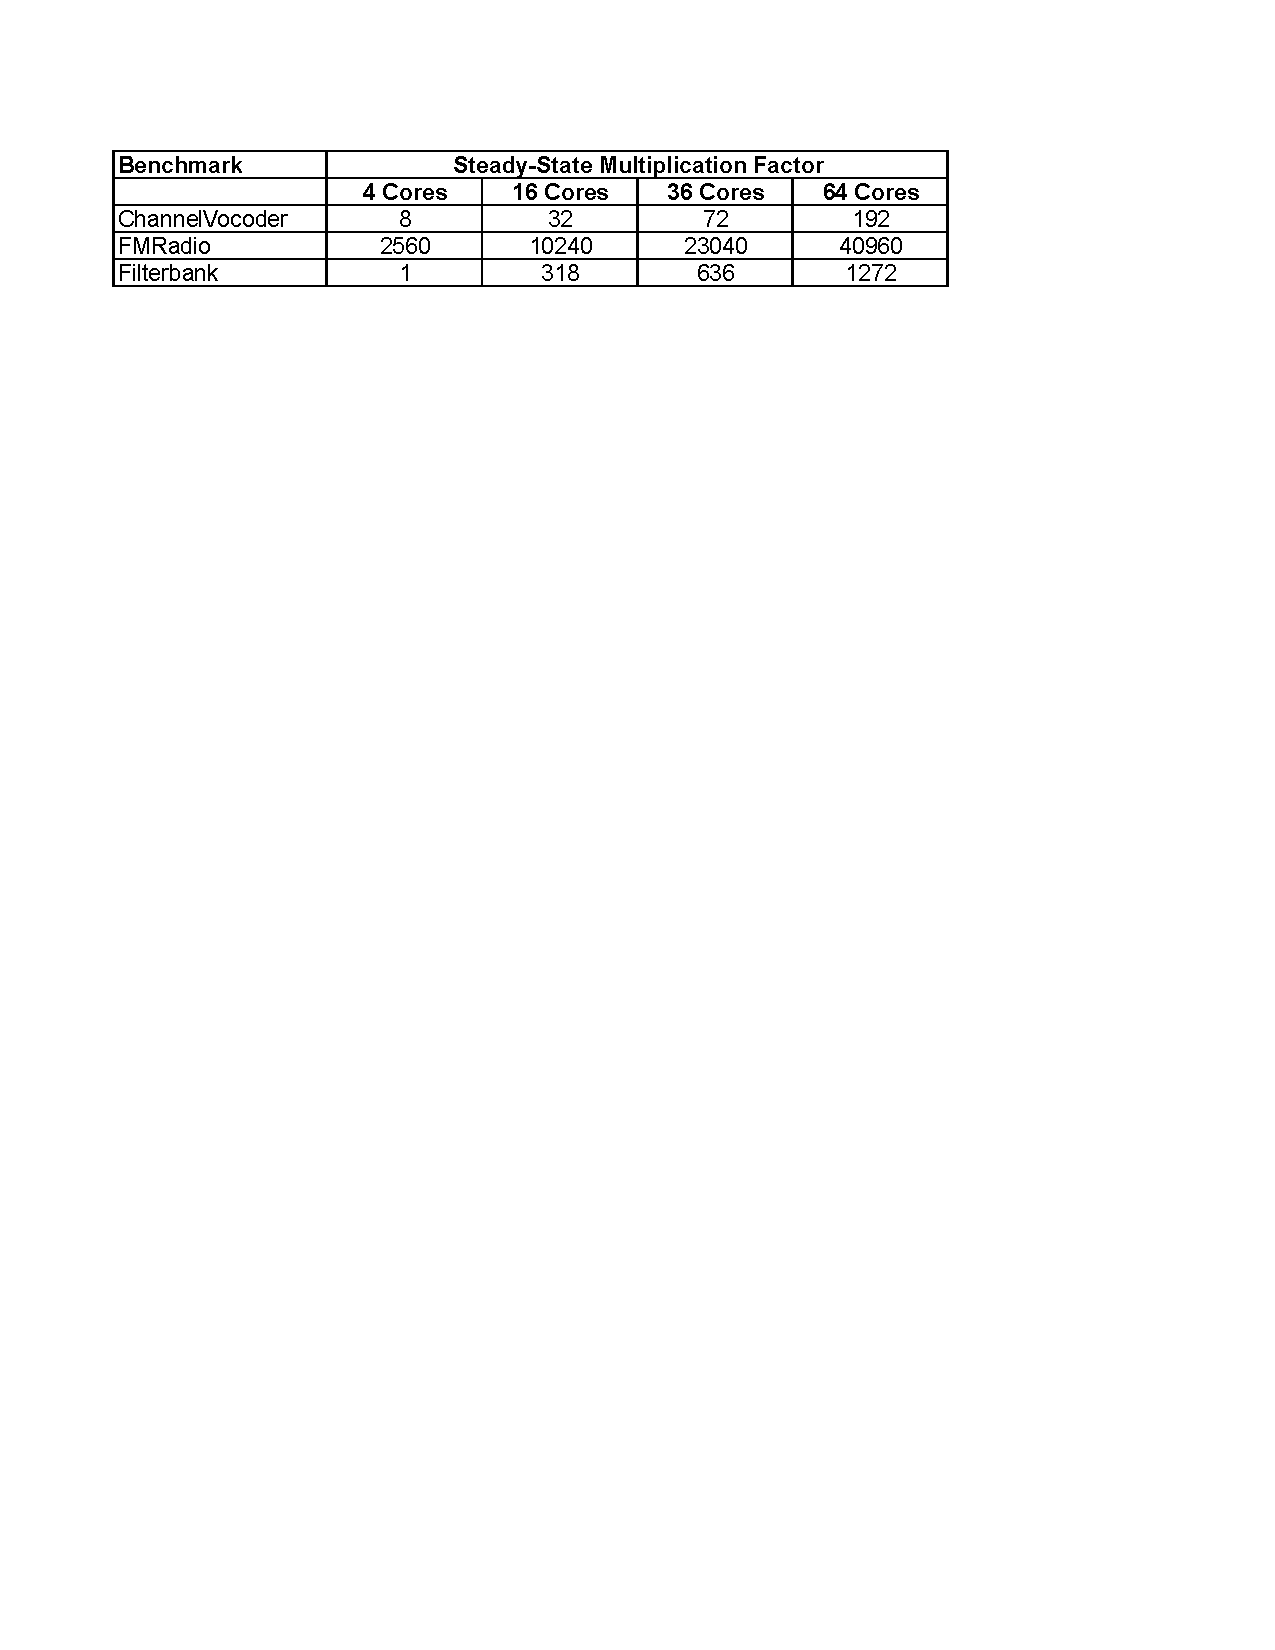
\includegraphics[width=3.7in]{figures/mult-table.pdf}} \\
\subfigure[]{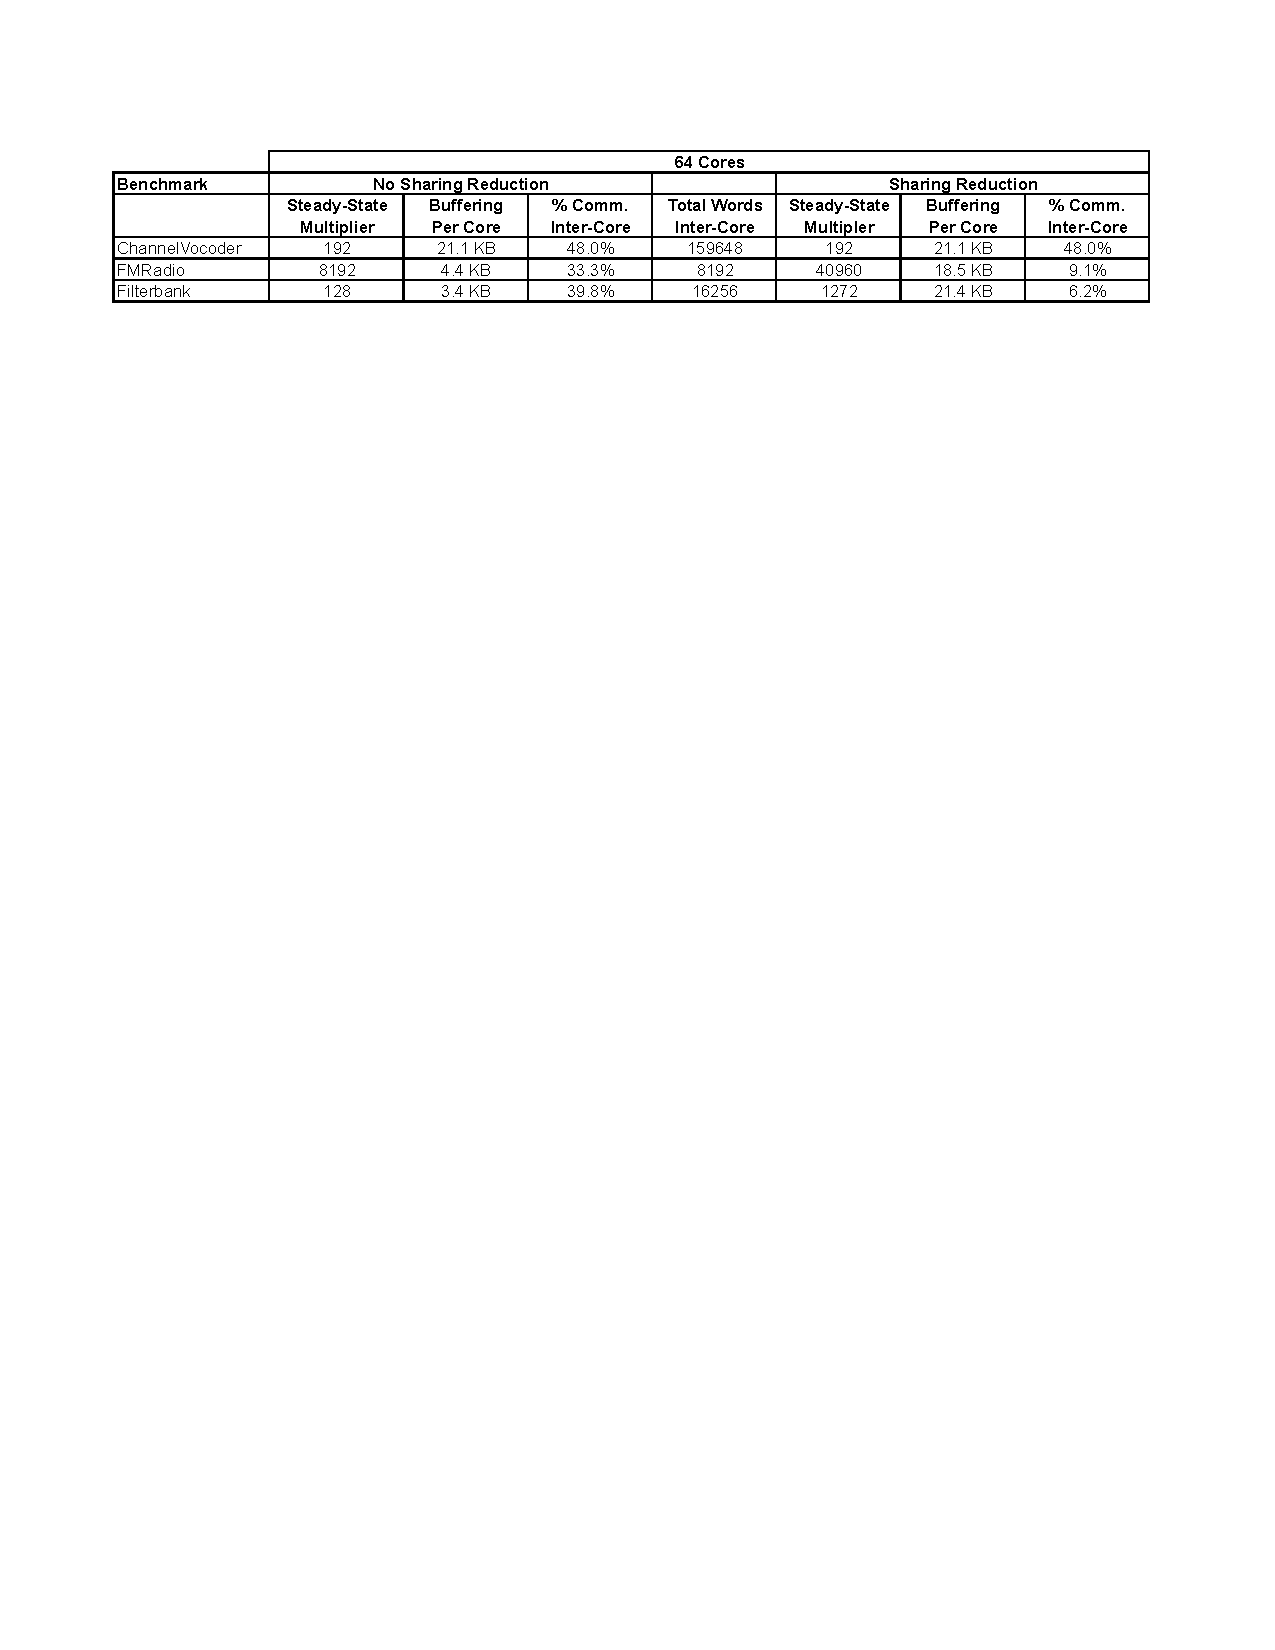
\includegraphics[width=6in]{figures/64-core-table.pdf}}
\caption[Communication, multiplier and buffering statistics for
benchmarks.]{
Communication, multiplier and buffering characteristics for
benchmarks: (a) gives the steady-state multipliers calculated for
sharing reduction, (b) compares the steady-state with and without
sharing reduction. 
\label{fig:fission-table}}
\end{figure*}

Figure~\ref{fig:fission-table}(a) gives the constant $c$
calculated for ChannelVocoder, Filterbank, and FMRadio for 4, 16, 36,
and 64 cores with: $T_{\mt{sharing}} = 0.10$ and $T_{\mt{apply}} =
0.05$.  The factor is larger for FMRadio because one filter
has $C(f) \gg o(S, f)$.  The multiplication factor affects both
latency and buffer sizes adversely.  The application designer will
have to decide if the latency of these techniques can be borne given
the application criteria.  The total buffering requirement is
increased when the steady-state is increased.  However, since we are
then fissing, the buffer is divided amongst the fission products, and
the {\it per-core} buffering requirement is unaffected by the
increase.  For example, FMRadio, has a per-core 18 KB buffering
requirement across all configurations (4, 16, 36, and 64 cores).  This
requirement fits in the per-core L2 size of 64 KB for the Tile64.

Figure~\ref{fig:fission-table}(b) compares the steady-state with and
without sharing reduction for a 64-core mapping.  For ChannelVocoder,
sharing reduction has no effect because most of the peeking filters do
not satisfy $T_{\mt{apply}} = 0.05$.  For the peeking filters that do,
the steady-state multiplier required for legal general fission for the
graph is enough to assure $T_{\mt{sharing}}$ is met.  Even though
sharing reduction has no effect for ChannelVocoder, general fission
avoids the 38\% of total items that were unnecessary duplicated by
dupdec.

For FMRadio and Filterbank, sharing reduction leads to significant
decreases in the percentage of total items communicated inter-core for
each steady-state.  The buffer requirement is increased an average of
5.2x for these benchmarks.  The total number of words communicated
inter-core during each steady-state is the same, with and without
sharing reduction.  However, the steady-state is greater in the
sharing reduction case, thus producing more outputs.

\begin{figure}[t]
\centering
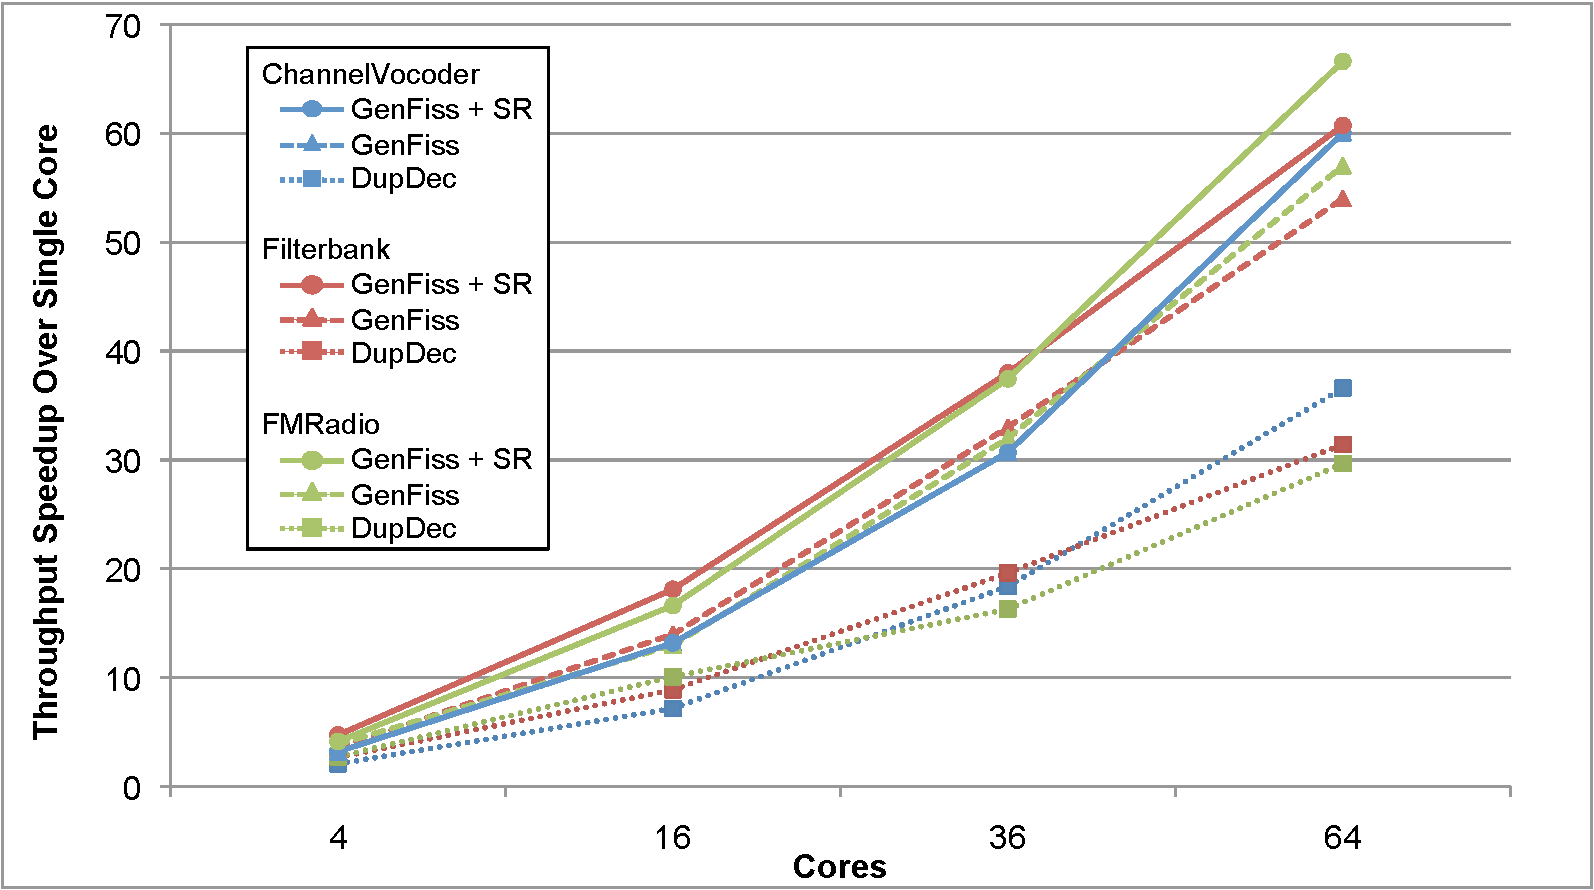
\includegraphics[width=3.3in]{figures/tilera-chart.pdf}
\caption[Comparing the fission techniques on the TILE64.]{
  Evaluation for dupdec versus general fission versus general fission with sharing reduction
  4, 16, 36, and 64 cores on the TILE64.  \label{fig:tilera-chart}}
\end{figure}

\begin{figure}[t]
\centering
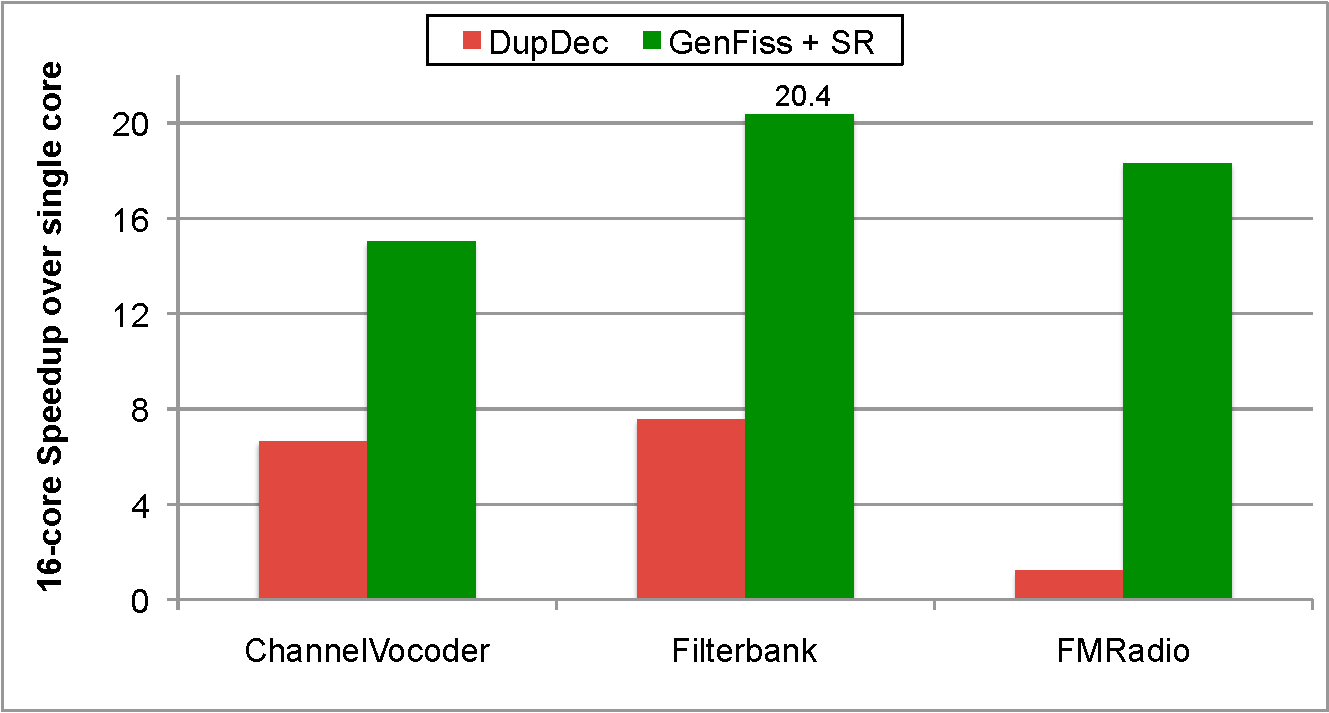
\includegraphics[width=3.3in]{figures/smp-chart.pdf}
\caption[Comparing the fission techniques on the 16-core SMP.]{
  Evaluation for dupdec versus general fission with sharing reduction
  for the 16-core SMP architecture.  \label{fig:smp-chart}}
\end{figure}

